\documentclass[12pt]{article}

\usepackage[utf8]{inputenc} %dla linuxa
\usepackage{polski} %polskie znaki takie jak "ę"
\usepackage{indentfirst} %pierwszy akapit tez bedzie mial wcięcie
\usepackage{wrapfig} % obrazek w tekście
\usepackage{array} % tabelki szerokość/wysokość
\usepackage{blkarray} % tabelki linie przerywane itp.
\usepackage{amsfonts} %to jest do tego, by zbiór liczba naturalnych miał fajne N
\usepackage{graphicx} %grafika
\usepackage{caption} % do montowania obrazkow
\title{Ironman Triathlon}
\author{Łukasz Ruzicki 271399}
\date{10.01.2020 r.}
\pagestyle{plain}


\begin{document}
\maketitle
\newpage

\tableofcontents

\newpage


\section{Triathlon}
\subsection{Co to jest?}
Triathlon to wielokrotna konkurencja polegająca na ukończeniu trzech ciągłych dyscyplin wytrzymałościowych. Choć wiele odmian sportu istnieje, triathlon w swojej najpopularniejszej formie obejmuje pływanie, jazdę na rowerze i bieganie w najbliższym czasie na różnych odległościach. Triathletes\footnote{Uczestnicy Triathlonu, czyli osoby biorące czynny udział w zawodach.} rywalizują o najszybszy czas zakończenia całego kursu, włącznie z "przejściami" z określonymi elementami pływania, cyklu i uruchamiania. Słowo "triathlon" ma pochodzenie greckie od trelc lub athlos.
\subsection{Jakie są rodzaje?}

Wyścigi triathlonów różnią się odległością. Według Międzynarodowej Unii Triatlonowej i Triatonu Stanów Zjednoczonych, główne międzynarodowe odległości wyścigowe to:
\begin{enumerate}

\item \textbf{Sprint Distance}; 750-metrowa pływalnia, 20-kilometrowy rower,\\ 5-kilometrowy bieg
\item \textbf{Średni dystans}; powszechnie określane jako "dystans olimpijski":\\ pływanie o długości 1,5 km, rower o długości 40 km, tor 10 km
\item \textbf{Długi kurs}; powszechnie określane jako 70,3 lub "pół-Ironman";\\ 1,9-kilometrowa pływalnia, 90-kilometrowy rower i 21,1 kilometrowa jazda
\item \textbf{Ultra Distance}; powszechnie określane jako 140.6 lub "Ironman";\\ 3,8-kilometrowa pływalnia, rower o długości 180,2 km, a 42.
\end{enumerate}
\begin{center}
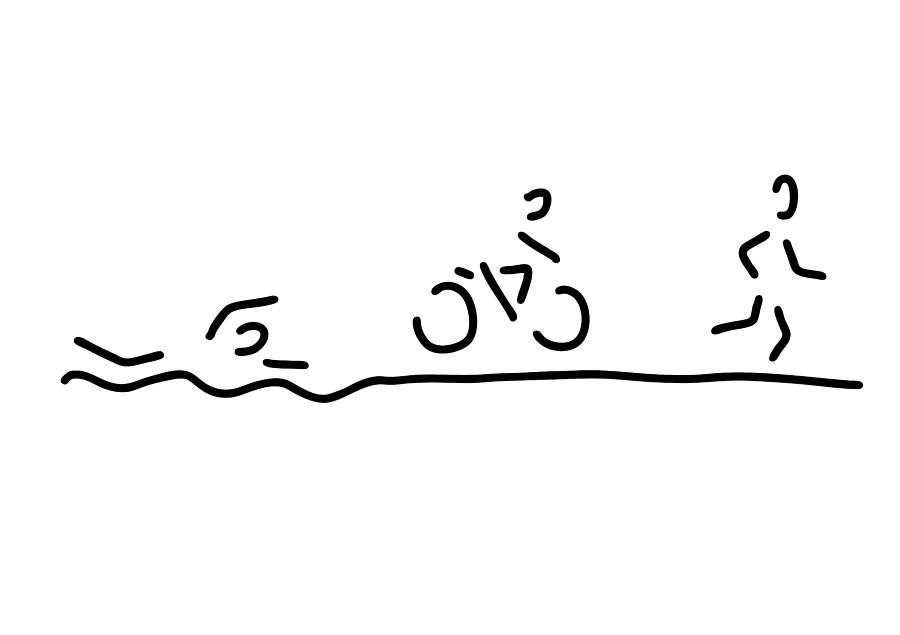
\includegraphics[width=0.28 \paperwidth]{dwa.jpg}
\end{center}

\section{Zawodnicy}
\subsection{Najsłynniejsi z Polski}


\begin{flushleft}
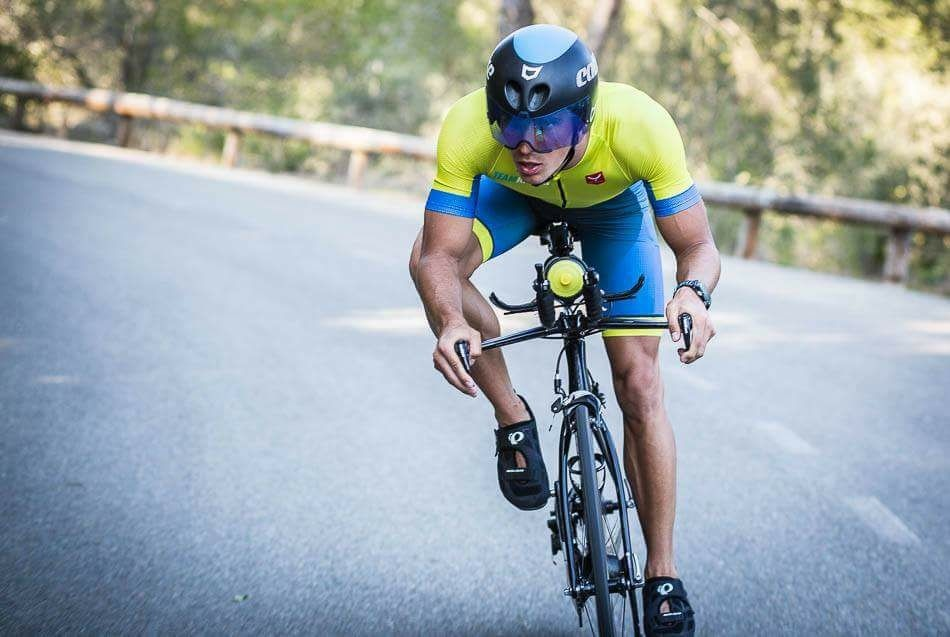
\includegraphics[width=0.3 \paperwidth]{jeden.jpg}
\end{flushleft}
\captionof{figure}{Robert Karaś, akutalny rekordzista podwójnego i potrójnego triathlonu.}

\begin{flushright}
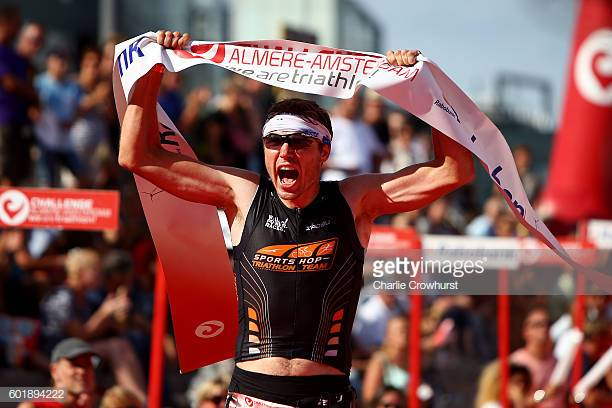
\includegraphics[width=0.3 \paperwidth]{trzy.jpg}
\end{flushright}
\captionof{figure}{Marek Jaskółka, czterokrotny mistrz Polski na dystansie olimpijskim.}

\begin{flushleft}
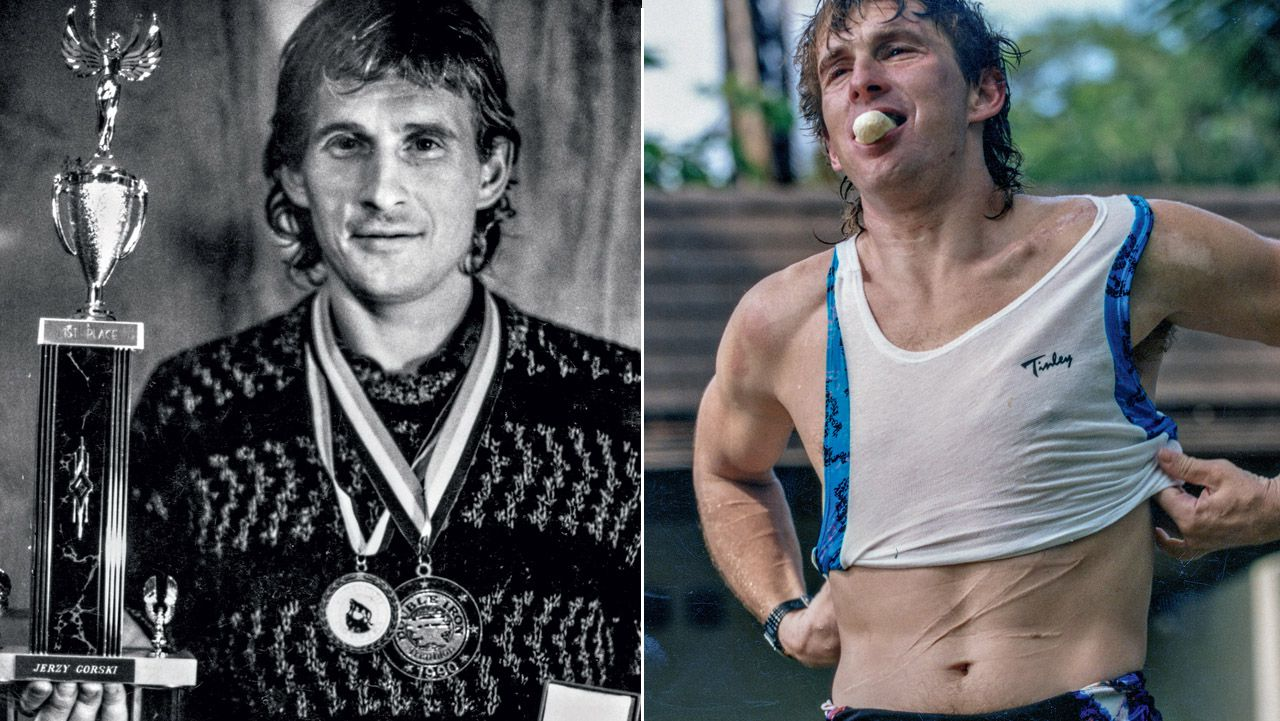
\includegraphics[width=0.3 \paperwidth]{cztery.jpg}
\end{flushleft}
\captionof{figure}{Jerzy Górski, wygrał Triathlon (podwójny Ironman) w Huntsville.}

\subsection{Światowi zawodnicy}

\begin{flushright}
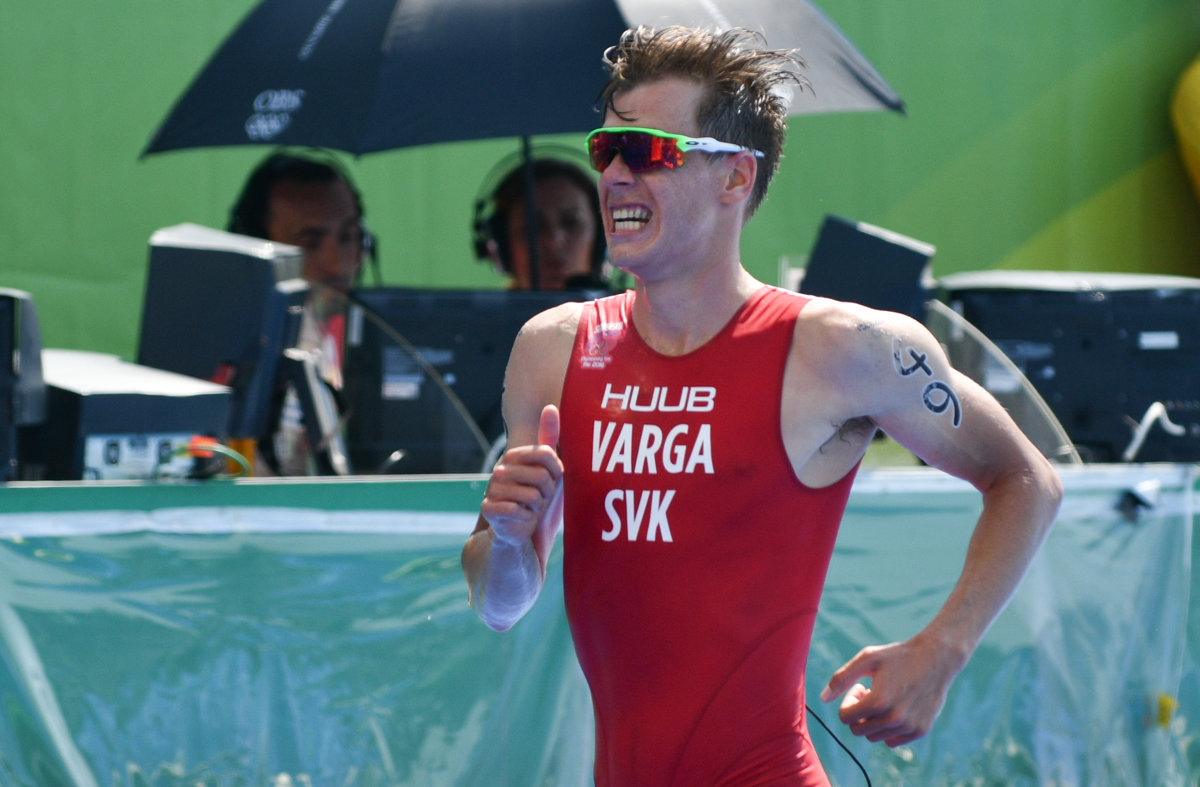
\includegraphics[width=0.3 \paperwidth]{piec.jpg}
\end{flushright}
\captionof{figure}{Richard Varga, najlepszy pływak z 2017 r.}

\begin{flushleft}
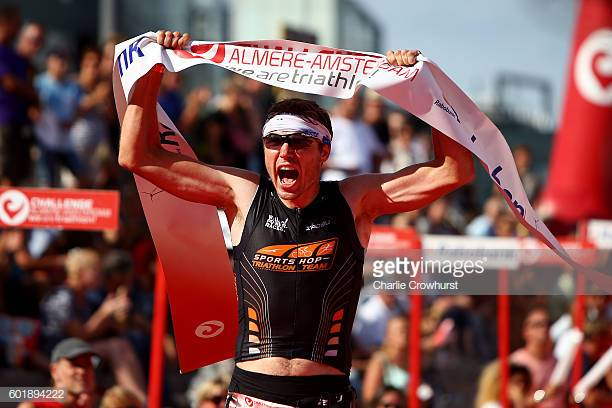
\includegraphics[width=0.3 \paperwidth]{trzy.jpg}
\end{flushleft}
\captionof{figure}{Alistair Brownlee, brat bliźniak Jonnego. Wraz z bratem stawał na podium.}

\begin{flushright}
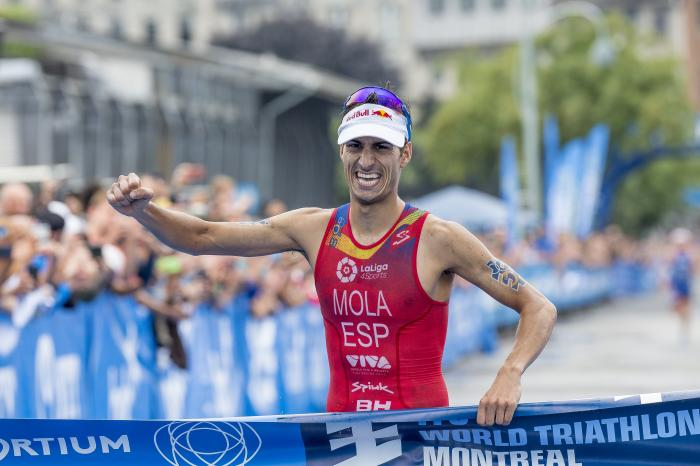
\includegraphics[width=0.3 \paperwidth]{siedem.jpg}
\end{flushright}
\captionof{figure}{Mario Mola, wielokrotny mistrz na odcinku biegowym.}

\section{Jak osiągnęli sukces?}
\subsection{Specjalna dieta}
\noindent \emph{Specjalna} dieta jest uważana za jedną z najważniejszych rzeczy dla zawodników. Mówi się, że stanowi ona \textbf{ 80\%} sukcesu sportowca. Bez dobrze dobranej diety, człowiek nie jest w stanie zapewnić odpowiednich składników swojemu ciału, aby to rozwijało się \cite{watzlawik83}.

\subsection{Waga}
\noindent Ponadto długodystansowcy muszą być \textit{wagi lekkiej}. Jest to bardzo ważny czynnik, który pozwala odciążyć i tak już obciążone stawy, które są wystawione na duże ryzyko podczas tak intensywnego i długiego wysiłku \cite{lukruz20}.
\subsection{Co jedzą?}

\noindent Dieta sportowca to wysokowartościowy posiłek, który zapewni odpowiednią dawkę energii zawodnikowi, aby ten był w stanie pokonać długie dystanse. Nie jest to proste, ponieważ człowiek może strawić do \textbf{300 kcal} podczas jednej\begin{wrapfigure}{r}{0.5\textwidth}
\begin{center}
\vspace{-20pt}

\includegraphics[width=0.35\textwidth]{osiem}
\end{center}
\vspace{-20pt}
\caption{{\scriptsize Sztućce, zbędne dla zawodników}}
\vspace{-10pt}
\end{wrapfigure}
 godziny, dlatego ważne jest, aby jeść w trakcie wykonywania wysiłku rzeczy, które szybko dostarczą energię i pozwolą na kontynuowanie wyzwania bez konieczności odpoczynku.

Jedzenie, które było źródłem energii do codziennych treningów nie sprawdza się na maratonach. Zawodnicy przy skrajnych wysiłkach potrafią nie przyjmować posiłków tylko dlatego, że nie mają na nie ochoty. Potrafią sobie zażyczyć przeróżne posiłki, które ich zespół musi spełnić, ponieważ pokarm trzeba przyjąć. Wielokrotnie na zawodach zdarzało się, że uczestnicy prosili na przykład o pizze Hawajską\footnote{Pizza z ananasem.} lub sushi \cite{aumann1992handbook}.
	 
{\footnotesize \textit{\textbf{Przykładowe posiłki sportowców zamieszczone są w tabeli na kolejnej stronie.}}}
\newpage
\begin{table}
\caption{Dieta Roberta Karasia na dzień przed zawodami}
\label{tab:Dieta na dzien przed zawodami}
\begin{center}
\setlength{\extrarowheight}{1pt}
\begin{tabular}{|c|l|c|c|}
\hline Posiłek & Nazwa & Ilość & Kalorie \\ \hline
1 & Risotto & 200 g & 198 \\ \hline
2 & Quasadilas & 200 g & 420 \\ \hline
3 & Łosoś & 150 g & 220 \\ \hline
4 & Małże & 220 g & 311\\ \hline
5 & Rosół & 250 ml & 140\\ \hline
\begin{tabular}{|l|c|r|}
\hline
6 & 7 & 8\\
\hline
\multicolumn{3}{|c|}{Wybór}\\ \hline
\end{tabular} & 

\begin{tabular}{|l|c|r|}
\hline
3BIT & Twix & Mars\\
\hline
\multicolumn{3}{|c|}{Kolejno}\\ \hline
\end{tabular} &

\begin{tabular}{|l|c|r|}
\hline
60 g & 70 g & 80 g\\
\hline
\multicolumn{3}{|c|}{Kolejno}\\ \hline
\end{tabular} &
\begin{tabular}{|l|c|r|}
\hline
88 & 87 & 90\\
\hline
\multicolumn{3}{|c|}{Kolejno}\\ \hline
\end{tabular} \\ \hline

\end{tabular}
\end{center}
\end{table}


\begin{table}
\caption{Posiłki w trakcie Triathlonu}
\label{Posiłki w trakcie Triathlonu}
\begin{center}
\setlength{\extrarowheight}{3pt}
\begin{tabular}{|l|c|c|c|c|c|c|c|c|c|c|} \BAhhline{|t===========|}
Pływanie (km) & \multicolumn{3}{|c|}{0,5} & \multicolumn{3}{|c|}{1,0} & \multicolumn{3}{|c|}{1,5} & 1,6 \\ \BAhhline{|...........|}
Posiłek & \multicolumn{3}{|c|}{3Bit} & \multicolumn{3}{|c|}{Snickers} & \multicolumn{3}{|c|}{Jabłko} & Redbull \\ \BAhhline{|===========|}
Cycling (km) & 4 & 8 & 12 & 16 & 20 & 24 & 28 & 32 & 36 & 40 \\ \BAhhline{|...........|}
Posiłek & \multicolumn{3}{|c|}{Redbull} & \multicolumn{4}{|c|}{Ale Gel} &Bpow & \multicolumn{2}{|c|}{Ale Gel} \\ \BAhhline{|===========|}
Bieganie (km) & \multicolumn{2}{|c|}{2} & \multicolumn{2}{|c|}{4} & \multicolumn{2}{|c|}{6} & \multicolumn{2}{|c|}{8} & \multicolumn{2}{|c|}{10} \\ \BAhhline{|...........|}
Posiłek & \multicolumn{6}{|c|}{Ale Gel Owocowy} & \multicolumn{2}{|c|}{3BIT} & \multicolumn{2}{|c|}{Bpow} \\ \BAhhline{|===========|}

\end{tabular}
\end{center}
\end{table}

\begin{center}

\includegraphics[width=0.3 \paperwidth]{bowl.png}
\end{center}

\section{Rzeczy niepotrzebne sportowcom}
\subsection{Wzory matematyczne na całki nieoznaczone}

\noindent {\large W}zory matematyczne na całki nieoznaczone są całkowicie zbędne przy profesjonalnym zajmowaniu się tym sportem, dlatego poniżej znajduję się lista wzorów, które nigdy w życiu nie będą użyteczne dla zawodnika. Ma to na celu pokazanie jakich rzeczy nie musi uczyć się sportowiec. Dla niektórych może być to część motywacji do działania
\cite{greenwade93}.

\begin{enumerate}
\item  $$f(x)=x^a \Rightarrow\int_{}^{} \frac{x^{a+1}}{a+1} \cdot dx$$

\item $$f(x)=sinx \Leftrightarrow \int_{}^{} \-cosx \cdot dx$$

\item $$f(x)=\frac{1}{cos^2x} \Leftrightarrow \int_{}^{} tgx \cdot dx$$

\item $$f(x)=\frac{-1}{\sqrt{1-x^2}} \Leftrightarrow \int_{}^{} arccosx \cdot dx$$
\end{enumerate}
\subsection{Własności}

\begin{itemize}

\item  $$\forall_{c \in R} \int_{}^{} c \cdot f(x),dx = c \int_{}^{} f(x), dx  $$

\item $$\forall_{c \in R} \int_{}^{} f(g(x)) \cdot g'(x), dx =  \int_{}^{} f(t) \cdot dt ; t=g(x), dt = g'(x) \cdot g(x)  $$

\end{itemize}

\subsection{Granica }

$$\exists_{x \in R} \lim_{x \to 0}\frac{x}{\log_a (x+1)}=lna$$
$$\sum_{i=1}^\infty X_i=i^2\cdot \frac{421^i}{i^i} \cdot i^2 \cdot lni$$


\listoffigures

\listoftables

\bibliographystyle{plain}
\bibliography{biblioteka}

\end{document}
